\documentclass{beamer}
\usepackage{tikz}
\date{Lundi 16 mai 2022}
\title{Attaque par saturation sur l'AES}
\author{Éloïse MERCADO-GARCIA \newline Vincent XAVIER \newline Clément LYONNET}

\begin{document}
	
	\begin{frame}
		[plain] \titlepage
	\end{frame}

	\begin{frame}
		\frametitle{Table des matières}
		\begin{itemize}
			\item Introduction
			\item AES-128
			\item Attaque par saturation
			\item Choix d'implémentation
			\item Démonstration
		\end{itemize}
	\end{frame}

	\begin{frame}
	    \frametitle{Introduction / Historique et Principe de l'attaque}
	    \begin{itemize}
	    	\item AES (Advanced Encryption Standard)
	        \item Créé par Joan Daemen et Vincent Rijmen
	        \item Standardisé en 2001
	        \item Algorithme de chiffrement par bloc, à clé symétrique
	        \vspace{0.5 cm}
	        \item Attaque par saturation sur l'AES à 4 tours.
	        \item Récupération de la clé à partir de 256 couples clairs-chiffrés.
	    \end{itemize}
	\end{frame}

\begin{frame}{AES-128 / Spécifications}
\begin{itemize}
    \item 4 opérations principales
    \begin{itemize}
        \item AddRoundKey
    \item SubBytes
    \item ShiftRows
    \item MixColumns
    \end{itemize}
    \item Taille du message : 128 bits
    \item Taille de la clé : 128 bits
    \item 10 tours
\end{itemize}
\end{frame}

\def\TABgen#1{
  \begin{array}{|c|c|c|c|} \hline
  #1_{0,0} & #1_{0,1} & #1_{0,2} & #1_{0,3} \\ \hline
  #1_{1,0} & #1_{1,1} & #1_{1,2} & #1_{1,3} \\ \hline
  #1_{2,0} & #1_{2,1} & #1_{2,2} & #1_{2,3} \\ \hline
  #1_{3,0} & #1_{3,1} & #1_{3,2} & #1_{3,3} \\ \hline
  \end{array}
}

\begin{frame}{AES-128 / Représentation}
    \begin{itemize}
    \item 128 bits = 16 octets
    \item Représenté sous forme d'une matrice d'octets 4 x 4
\end{itemize}
    \vspace{0.5 cm}
    \centering 
    $$ \TABgen{a} $$
\end{frame}

\begin{frame}{AES-128 / Algorithme}
\centering
    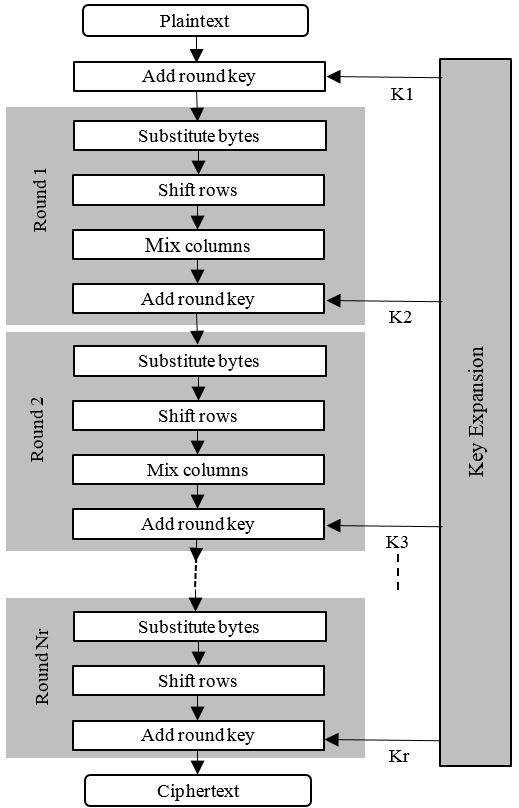
\includegraphics[width=0.5\textwidth]{images/Advanced-Encryption-Standard-AES-Algorithm.jpg}
\end{frame}

\begin{frame}{AES-128 / AddRoundKey}
\begin{itemize}
    \item Clé de 128 bits
    \item 11 sous-clés pour les 10 tours
\end{itemize}
	\vspace{0.5 cm}
    \centering
    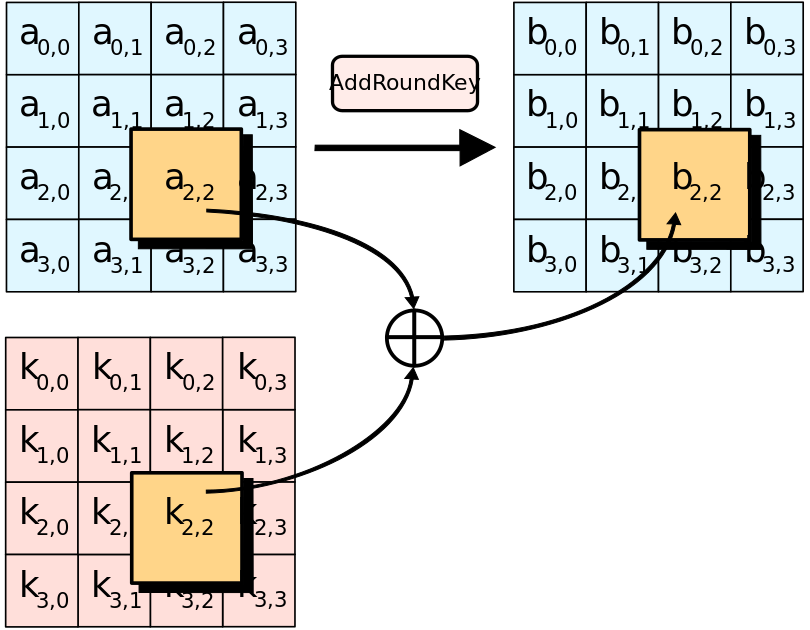
\includegraphics[width=0.6\textwidth]{images/AES-AddRoundKey.png}
\begin{itemize}
    \item Exemple : $ \text{1}8_{16} (00011000) \bigoplus 82_{16} (10000010) $\\
    $\longrightarrow 9\text{A}_{16} (10011010) $ \\ 
\end{itemize}
\end{frame}

\begin{frame}{AES-128 / SubBytes}
\begin{itemize}
    \item S-box ( table de substitution )
    \item Fournit la non-linéralité dans le chiffrement
\end{itemize}
    \vspace{0.5 cm}
    \centering
    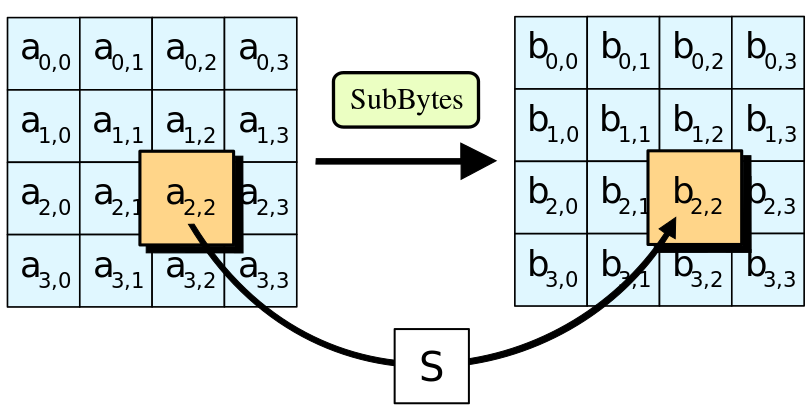
\includegraphics[width=0.7\textwidth]{images/AES-SubBytes.png}
\end{frame}

\begin{frame}{AES-128 / SubBytes - S-box}
    \centering
    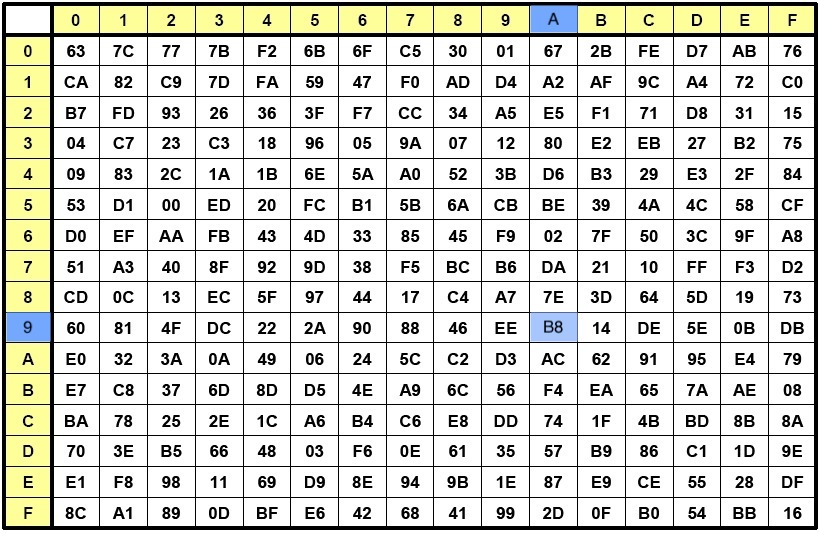
\includegraphics[width=0.7\textwidth]{images/AES_Sbox.jpg}
    \begin{itemize}
		\item  Exemple : $9\text{A}_{16} \longrightarrow \text{B}8_{16} $
	\end{itemize}
\end{frame}

\begin{frame}{AES-128 / ShiftRows}
    \begin{itemize}
        \item Une permutation circulaire vers la gauche
        \item 1ère ligne reste inchangée
        \item 2ème, 3ème et 4ème sont décalés respectivement de 1, 2 et 3
    \end{itemize}
    \vspace{0.5 cm}
    \centering
    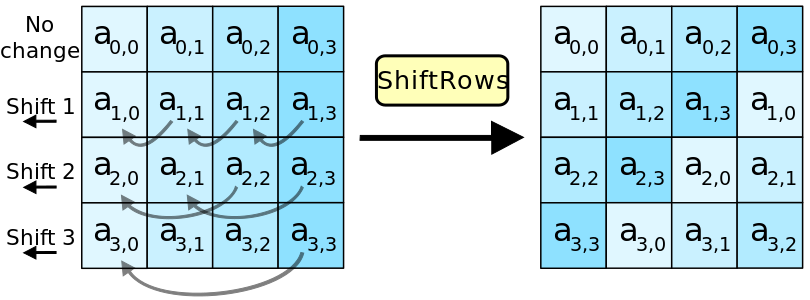
\includegraphics[width=0.8\textwidth]{images/AES-ShiftRows.png}
    \begin{itemize}
        \item Pour éviter que les colonnes soient chiffrées indépendamment (cf MixColumns)
    \end{itemize}
\end{frame}

\def\MixColumn{\begin{pmatrix} 
  2 & 3 & 1 & 1 \\ 
  1 & 2 & 3 & 1 \\ 
  1 & 1 & 2 & 3 \\ 
  3 & 1 & 1 & 2 \\ 
  \end{pmatrix}}
 
\def\colonne#1{
 \begin{pmatrix}
  #1_{0,i} \\
  #1_{1,i} \\
  #1_{2,i} \\
  #1_{3,i}
  \end{pmatrix}
}

\begin{frame}{AES-128 / MixColumns}
\begin{itemize}
    \item Multiplication d'une colonne avec une matrice
\end{itemize}
\vspace{0.5 cm}
    \centering
    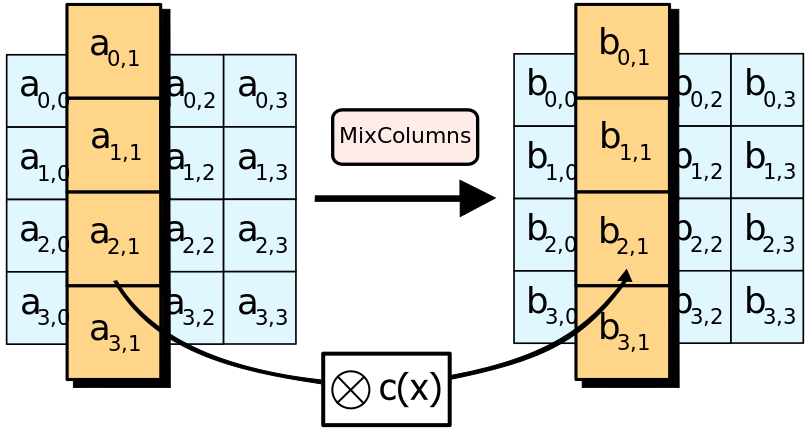
\includegraphics[width=0.7\textwidth]{images/AES-MixColumns.png}
    \begin{itemize}
    \item Avec ShiftRows, MixColumns assure la diffusion dans le chiffrement (effet avalanche).
\end{itemize}
\end{frame}

\begin{frame}{AES-128 / MixColumns}
\begin{itemize}
    \item c(x) $\longrightarrow$ Matrice 4 x 4
\end{itemize}
\vspace{0.5 cm}
    $$ \colonne{a} \otimes \MixColumn = \colonne{b} \quad $$
    \centering
   $$ \text{ avec } i \in [0,3] \text { représentant la colonne }$$
   \begin{itemize}
   \item Une multiplication avec modulo $$I(x) = X^8 + X^4 + X^3 + X + 1$$
    \item On répète donc le processus 4 fois
\end{itemize}
\end{frame}


\begin{frame}{AES-128 / KeyExpansion}
	\begin{itemize}
		\item 10 sous-clés sont créés
	\end{itemize}
	$$
	\begin{array}{c c}
		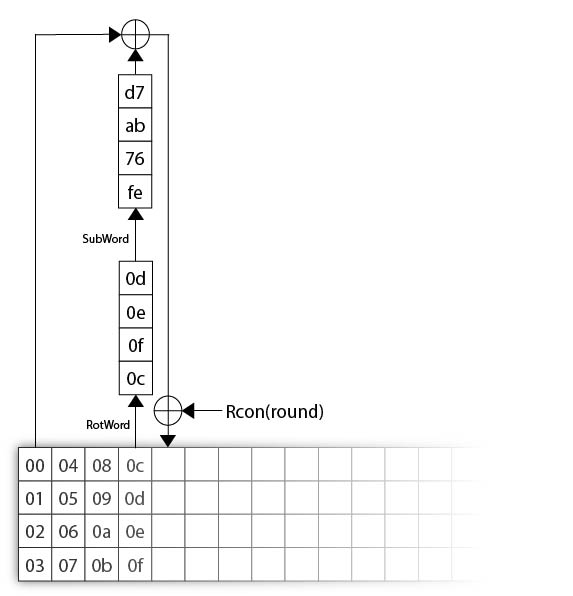
\includegraphics[width=.5\textwidth]{images/KS.jpg} &
		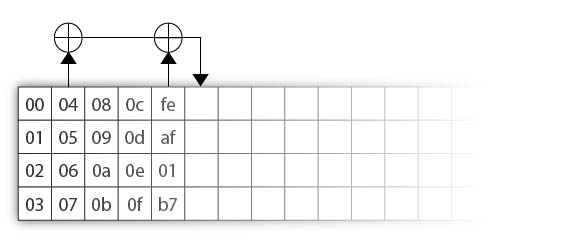
\includegraphics[width=0.45\textwidth]{images/KS1.jpg}
	\end{array}
	$$
	\begin{itemize}
		\item KeyExpansion est réversible.
	\end{itemize}
\end{frame}

	\begin{frame}
		\frametitle{Attaque par saturation}
		
		\begin{itemize}
			\item Découverte par Lars Knudsen et David Wagner en 2002.
   			\item Objectif : retrouver la clé de chiffrement.
      		\item Attaque possible sur une version simplifiée de l'AES : l'AES-128 4 tours dans le cadre de ce projet.
        	\item Type d'attaque : clair choisi.
		\end{itemize}
		\vspace{0.5 cm}
		$$
		\begin{array}{c c c}
			AES_{K}(m_0) & = & c_0 \\
			AES_{K}(m_1) & = & c_1 \\
			& \vdots & \\
			AES_{K}(m_{255}) & = & c_{255} \\
		\end{array}
		$$
	\end{frame}

	\begin{frame}
		\frametitle{Attaque par saturation}
		 \begin{itemize}
			\item Représentation de 128 bits pour AES :
			$$
			\begin{array}{|c|c|c|c|}
				\hline
				1 & 2 & 3 & 4 \\
				\hline
				5 & 6 & 7 & 8 \\
				\hline
				9 & 10 & 11 & 12 \\
				\hline
				13 & 14 & 15 & 16 \\
				\hline
			\end{array}
			$$
			\item Intégrale dans le cadre de l'attaque : 
			$$
			\mathcal{I}_j = \bigoplus_{i=0}^{255}\ \mathcal{M}_{j}^{i}
			$$
			Avec $\mathcal{M}_{j}^{i}$ l'octet j de la i\textsuperscript{ème} matrice $4 \times 4$.
		 \end{itemize}
	\end{frame}

	\begin{frame}
		\frametitle{Attaque par saturation}
		\begin{itemize}
			\item Distingueur
			\begin{itemize}
				\item Utilisé pour faire apparaitre des propriétés mathématiques.
				\item Les propriétés du distingueur : $\mathcal{A},\ \mathcal{C},\ \mathcal{S}\ et\ ?.$
    			\item Permet de retrouver la dernière sous-clé octet par octet.
       			\item Dirige le choix de l'attaquant :
			\end{itemize}
		\end{itemize}
		\vspace{0.5 cm}
			$$
			\begin{array}{|c|c|c|c|}
				\hline
				\mathcal{A} & \mathcal{C} & \mathcal{C} & \mathcal{C} \\
				\hline
				\mathcal{C} & \mathcal{C} & \mathcal{C} & \mathcal{C} \\
				\hline
				\mathcal{C} & \mathcal{C} & \mathcal{C} & \mathcal{C} \\
				\hline
				\mathcal{C} & \mathcal{C} & \mathcal{C} & \mathcal{C} \\
				\hline
			\end{array}
			$$
			\vspace{0.5 cm}
			Distingueur dû au choix des couples clair-chiffré de l'attaquant.
	\end{frame}

	\begin{frame}
		\frametitle{Attaque par saturation}
		Transformation du distingueur avant le premier tour :
		\begin{figure}
			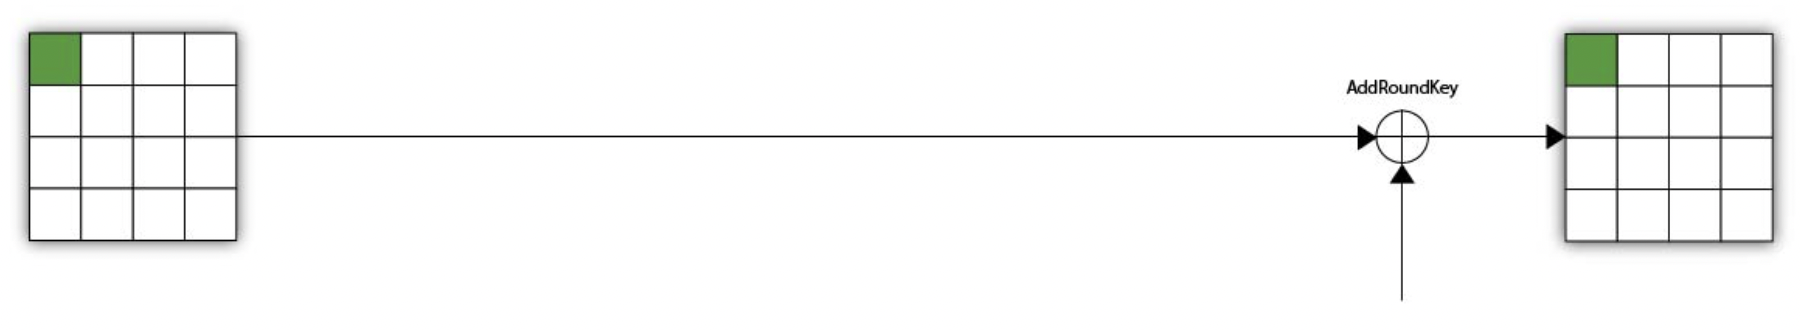
\includegraphics[width=1\textwidth]{images/AES_round_0.png}
			\caption{
				{\scriptsize
					{\color{green} Vert $\rightarrow$ $\mathcal{A}$},
					Blanc $\rightarrow$ $\mathcal{C}$,
				}
			}
		\end{figure}
	\end{frame}

	\begin{frame}
		\frametitle{Attaque par saturation}
		Transformation du distingueur lors du premier tour :
		\begin{figure}
			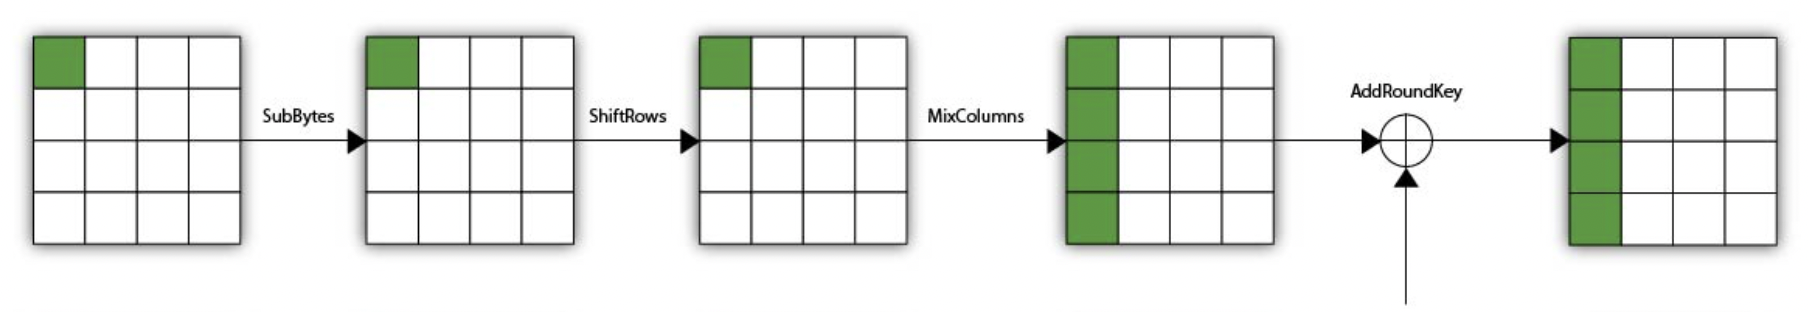
\includegraphics[width=1\textwidth]{images/AES_round_1.png}
			\caption{
				{\scriptsize
					{\color{green} Vert $\rightarrow$ $\mathcal{A}$},
					Blanc $\rightarrow$ $\mathcal{C}$,
				}
			}
		\end{figure}
	\end{frame}

	\begin{frame}
		\frametitle{Attaque par saturation}
		Transformation du distingueur lors du deuxième tour :
		\begin{figure}
			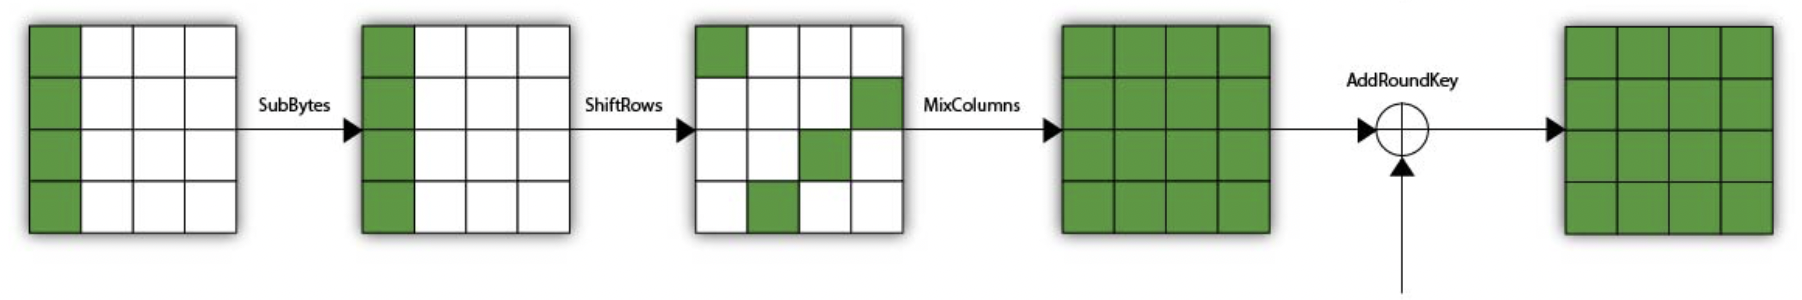
\includegraphics[width=1\textwidth]{images/AES_round_2.png}
			\caption{
				{\scriptsize
					{\color{green} Vert $\rightarrow$ $\mathcal{A}$},
					Blanc $\rightarrow$ $\mathcal{C}$,
				}
			}
		\end{figure}
	\end{frame}

	\begin{frame}
		\frametitle{Attaque par saturation}
		Transformation du distingueur lors du troisième tour :
		\begin{figure}
			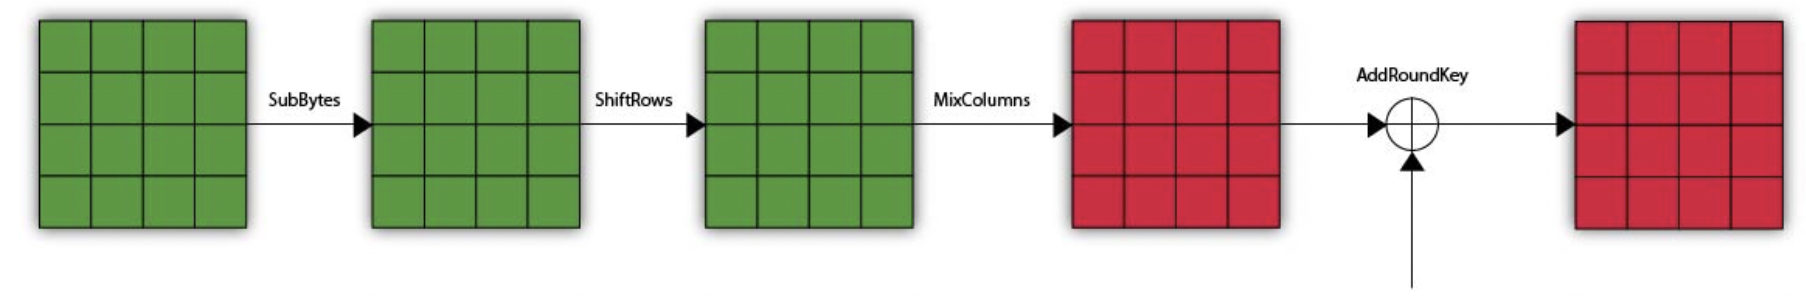
\includegraphics[width=1\textwidth]{images/AES_round_3.png}
			\caption{
				{\scriptsize
					{\color{green} Vert $\rightarrow$ $\mathcal{A}$},
					{\color{red} Rouge $\rightarrow$ $\mathcal{S}$},
				}
			}
		\end{figure}
	\end{frame}

	\begin{frame}
		\frametitle{Attaque par saturation}
		Transformation du distingueur lors du quatrième tour :
		\begin{figure}
			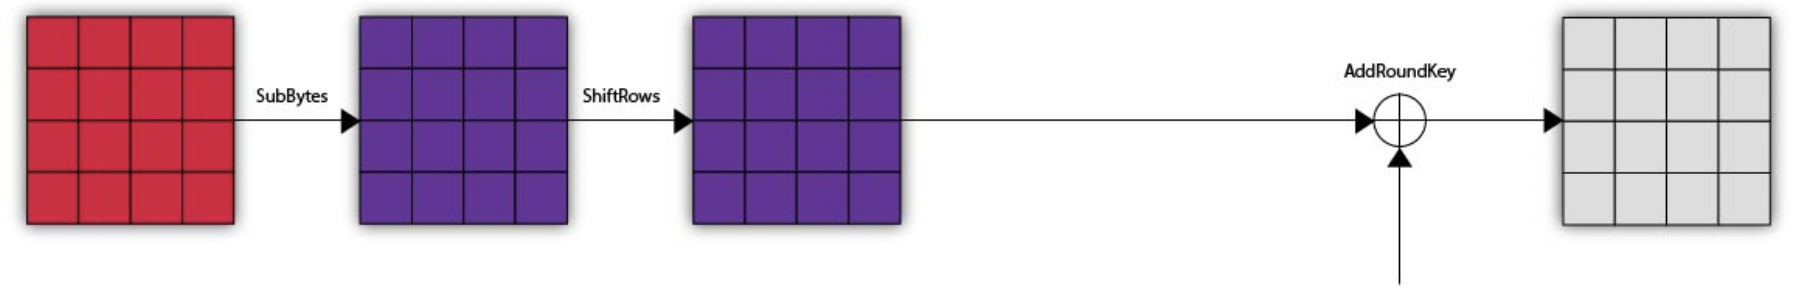
\includegraphics[width=1\textwidth]{images/AES_round_4.png}
			\caption{
				{\scriptsize
					{\color{red} Rouge $\rightarrow$ $\mathcal{S}$},
					{\color{violet} Violet $\rightarrow$ ?}
				}
			}
		\end{figure}
	\end{frame}

	\begin{frame}
		\frametitle{Attaque par saturation}
		\begin{figure}
			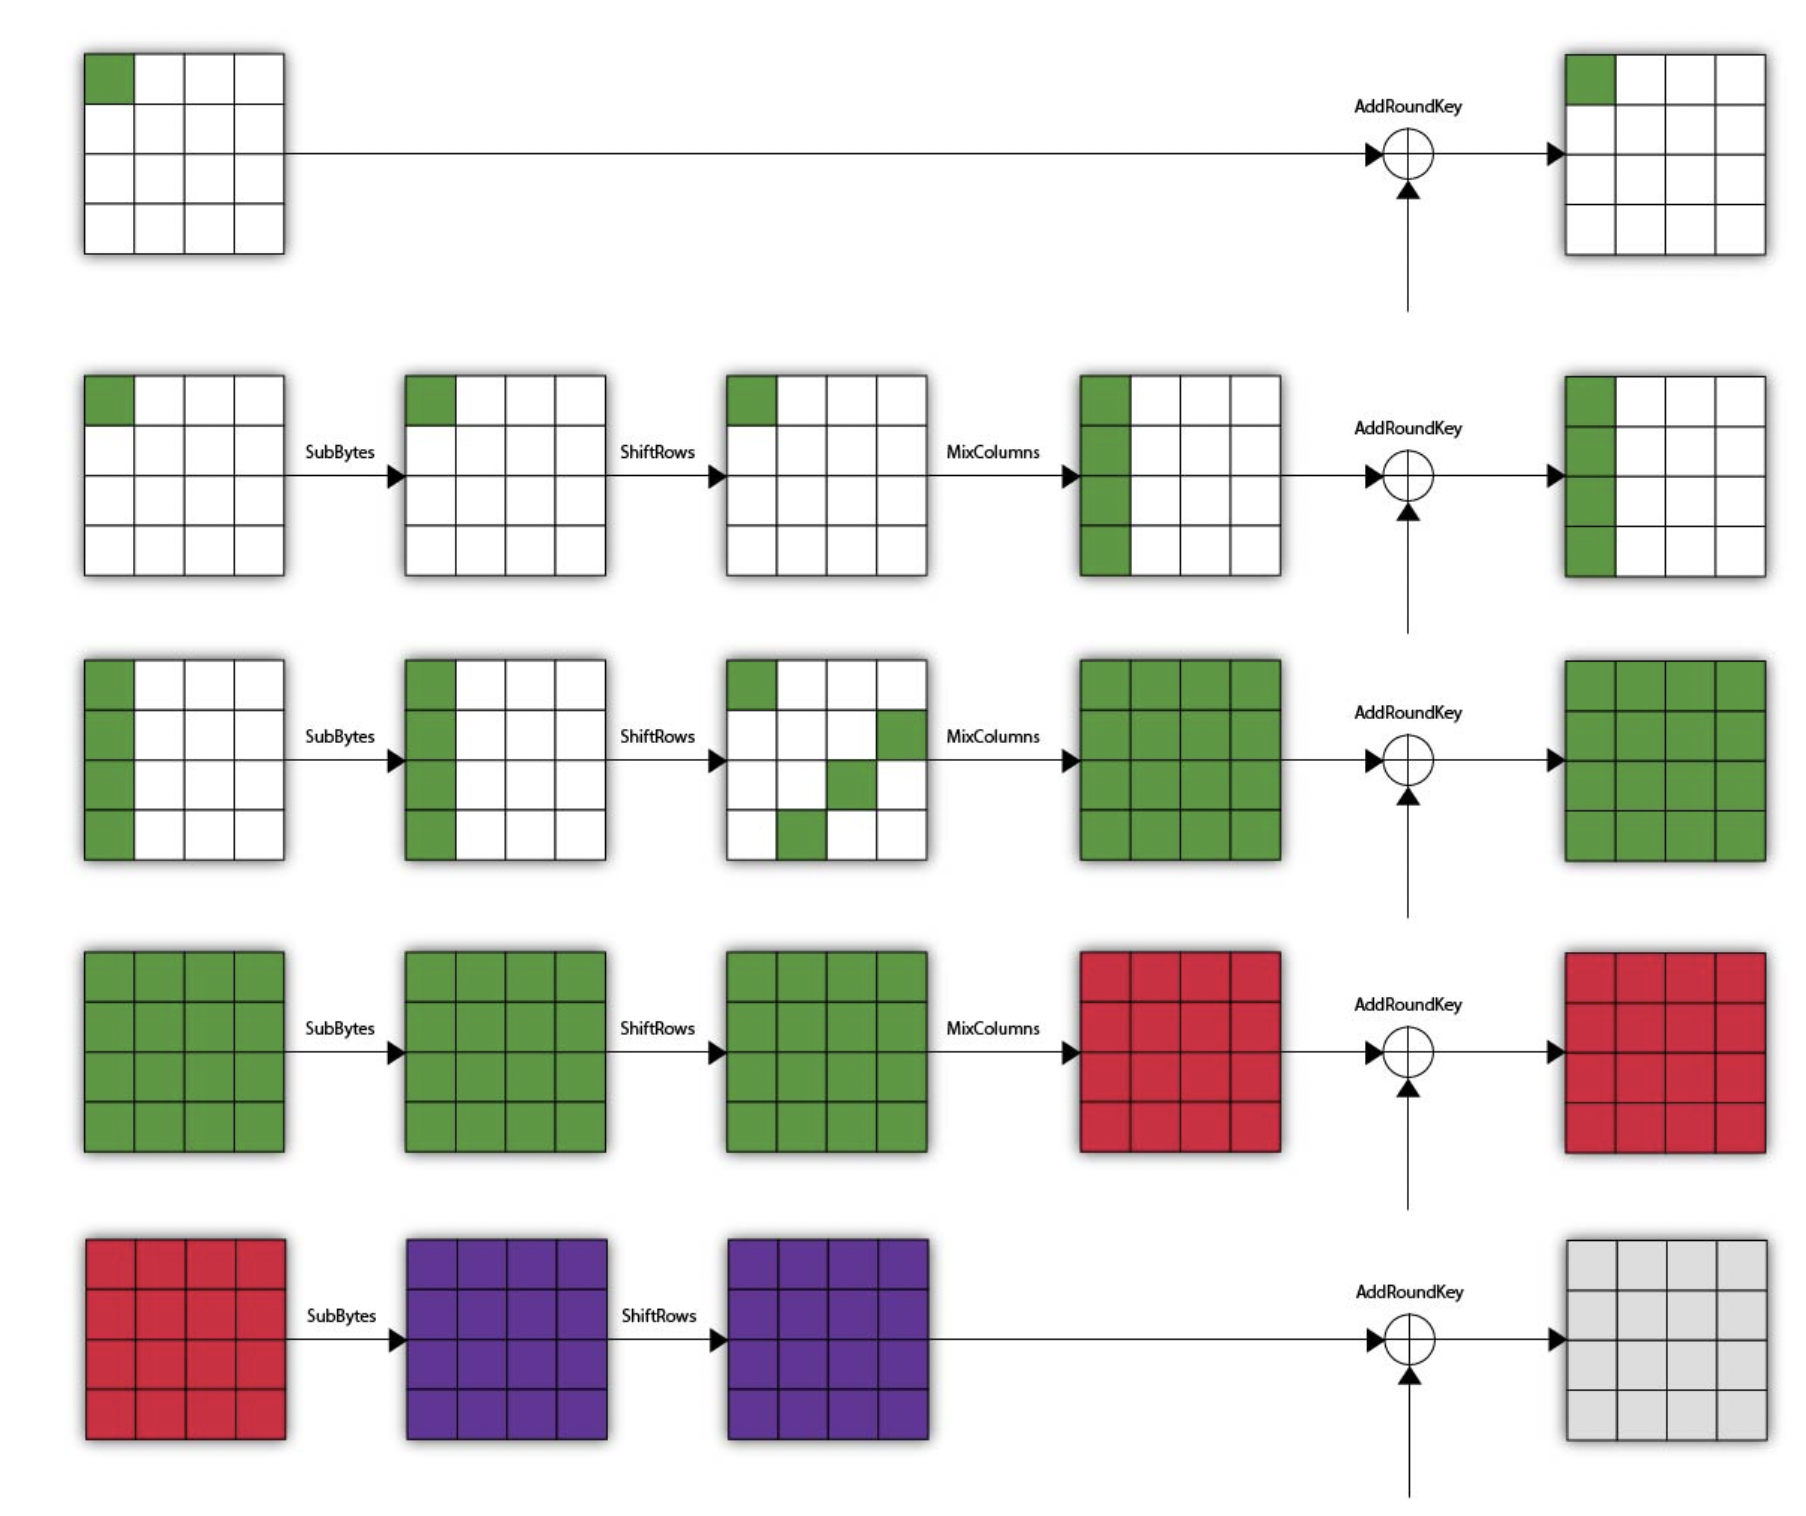
\includegraphics[width=0.75\textwidth]{images/AES_distingueur.png}
			\caption{
				{\scriptsize
					{\color{green} Vert $\rightarrow$ $\mathcal{A}$},
					Blanc $\rightarrow$ $\mathcal{C}$,
					{\color{red} Rouge $\rightarrow$ $\mathcal{S}$},
					{\color{violet} Violet $\rightarrow$ ?}
				}
			}
		\end{figure}
	\end{frame}

	\begin{frame}
		\frametitle{Attaque par saturation}
		Utilisation de la récursivité pour retrouver la dernière sous-clé :
		{\centering
		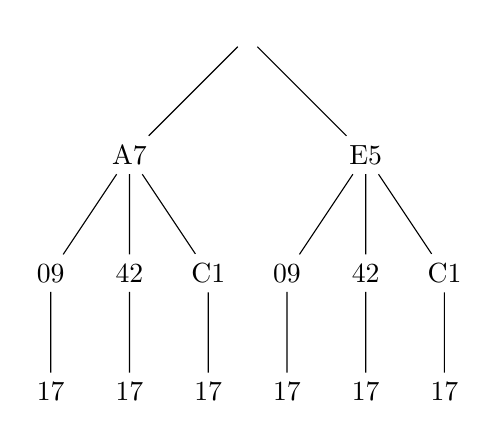
\begin{tikzpicture}
			[
				level 1/.style = {sibling distance = 3cm},
				level 2/.style = {sibling distance = 1cm}
			]
			\node {}
				child 
				{ node {A7}
					child 
					{ node {09}
						child {node {17}}
					}
					child 
					{ node {42}
						child {node {17}}
					}
					child 
					{ node {C1}
						child {node {17}}
					}
				} 
				child 
				{ node {E5}
					child 
					{ node {09}
						child {node {17}}
					}
					child 
					{ node {42}
						child {node {17}}
					}
					child 
					{ node {C1}
						child {node {17}}
					}
				};
			\end{tikzpicture} \\ }
			Le premier octet de la dernière sous-clé possède 2 valeurs candidates, le deuxième octet a 3 valeurs candidates, le troisième a 1 valeur...
	\end{frame}

	\begin{frame}
		\frametitle{Attaque par saturation}
		\begin{itemize}
			\item L'attaquant utilise 3 ensembles de couple différents ($256 \times 3$), avec une constante différente pour chaque ensemble.
			\item Il calcule les 16 listes d'octets candidats de chacun des trois ensembles.
   			\item Il fait l'intersection de chaque liste et retrouve ainsi la valeur de la dernière sous-clé.
			\begin{itemize}
				\item Intersection des trois listes numéro 1,
				\item Intersection des trois listes numéro 2,
				\item ...
			\end{itemize}
		\end{itemize}
	\end{frame}

	\begin{frame}
		\frametitle{Choix d'implémentation}
		\begin{itemize}
			\item Langage de programmation
			\item Type utilisé
			\item Modes d'exécution
			\item CTR
			\item Gestions d'erreurs
		\end{itemize}
	\end{frame}

	\begin{frame}
		\frametitle{Conclusion}
		\begin{itemize}
			\item Améliorations possibles :
			\begin{itemize}
				\item Interface graphique
    			\item Optimisation de code pour plus de rapidité
       			\item Extension de l'attaque pour l'AES 5 tours, 6 tours...
			\end{itemize}
		\end{itemize}
	\end{frame}

\end{document}

